\documentclass{article}
\usepackage[utf8]{inputenc}

\title{EE2703: Assignment 10}
\author{Yogesh Agarwala \\ EE19B130}
\date{June 3, 2021}

\usepackage{natbib}
\usepackage{graphicx}
\usepackage{amsmath}
\usepackage{listings}

\begin{document}

\maketitle

\section*{Introduction}
In this assignment, we explore the nature of DFTs of non periodic signals,
and the use of DFT in parameter estimation. These non-periodic functions have a discontinuity when periodically extended. The discontinuity lead to non-harmonic components in the FFT which decay as
\(\frac{1}{\omega}\), due to Gibbs phenomenon. We resolve this problem using a hamming window. We use this windowed transform to analyse signals known to contain a sinusoid of unknown frequencies and extract its phase and frequency. We also perform a sliding DFT on a chirped signal and plot the results.

\clearpage

\section {Examples}

\subsection{Spectrum of $y=\sin\left(\sqrt{2} \times t\right)$ over $-\pi$ to $+\pi$ with 64 samples}

\begin{figure}[h!]
\centering
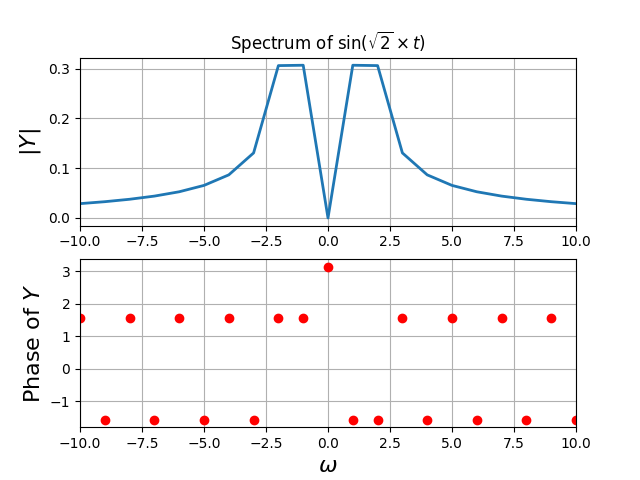
\includegraphics[scale=0.5]{Figure_1.png}
\caption{Spectrum of $sin(\sqrt{2}t)$}
\label{fig:universe}
\end{figure}

\subsection{$y=\sin\left(\sqrt{2} t\right)$ over several time periods b/w $-3\pi$ \& $3\pi$}
Original function for which we want the DFT:
\begin{figure}[h!]
\centering
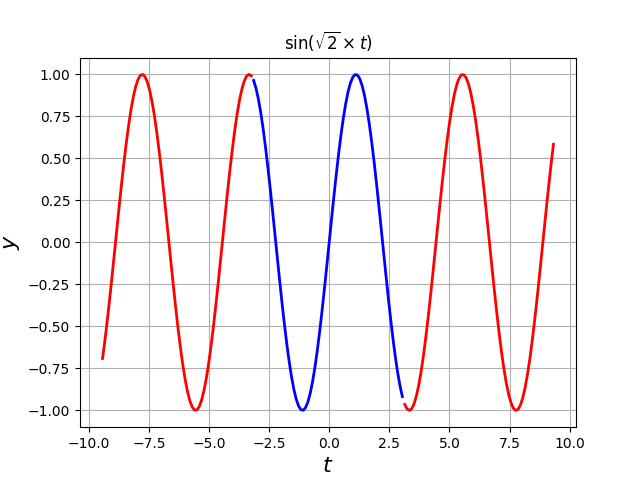
\includegraphics[scale=0.5]{Figure_2.png}
\caption{$sin(\sqrt{2}t)$}
\label{fig:universe}
\end{figure}

\newpage

\subsection{$y=\sin\left(\sqrt{2}\times t\right)$ with $t$ wrapping every $2\pi$}

Since the DFT is computed over a finite time interval, We actually plotted the DFT for this function
\begin{figure}[h!]
\centering
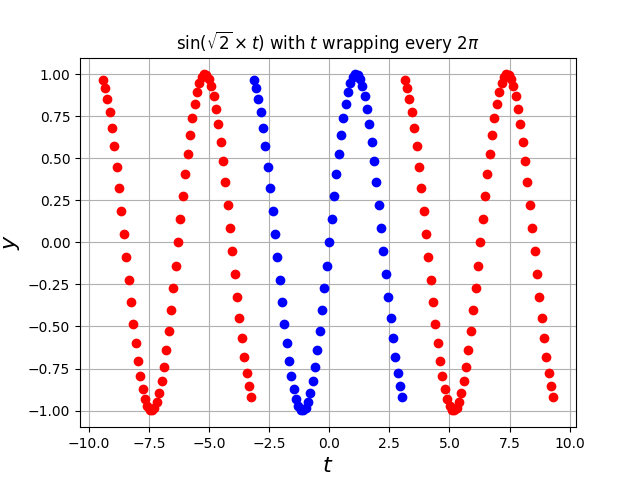
\includegraphics[scale=0.5]{Figure_3.png}
\caption{Spectrum of $sin(\sqrt{2}t)$}
\label{fig:universe}
\end{figure}

\subsection{Digital ramp}

The above discontinuities lead to  non harmonic components in the FFT which decay as \(\frac{1}{\omega}\). To confirm
this, we plot the spectrum of the periodic ramp below:
\begin{figure}[h!]
\centering
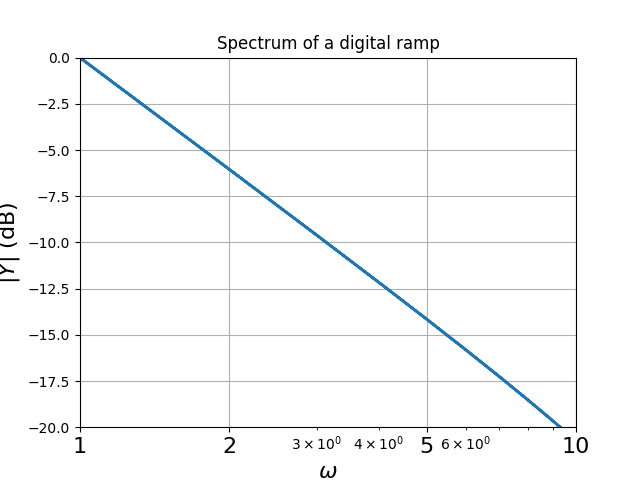
\includegraphics[scale=0.5]{Figure_4.png}
\caption{Spectrum of $sin(\sqrt{2}t)$}
\label{fig:universe}
\end{figure}

\subsection{Windowing}
The hamming window removes discontinuities by attenuating the high frequency components that cause the discontinuities.
The hamming window function is given by
\begin{equation}
    x[n] = 0.54 + 0.46cos(\frac{2\pi n}{N-1})
\end{equation}


We now multiply our signal with the hamming window and periodically extend it. Note that the discontinuities nearly vanish
\begin{figure}[h!]
\centering
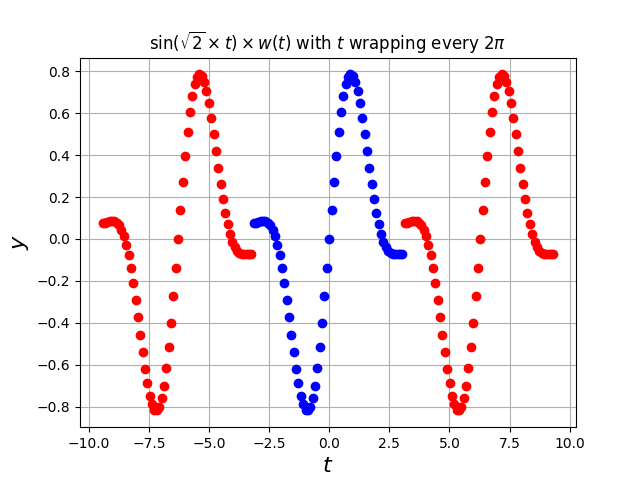
\includegraphics[scale=0.6]{Figure_5.png}
\caption{Spectrum of $sin(\sqrt{2}t)*w(t)$}
\label{fig:universe}
\end{figure}
\clearpage

\subsection{$y=\sin\left(\sqrt{2}\times t\right)\times w(t)$ with $t$ wrapping every $2\pi$}

The spectrum that is obtained with a time period $2\pi$ is given below:
\begin{figure}[h!]
\centering
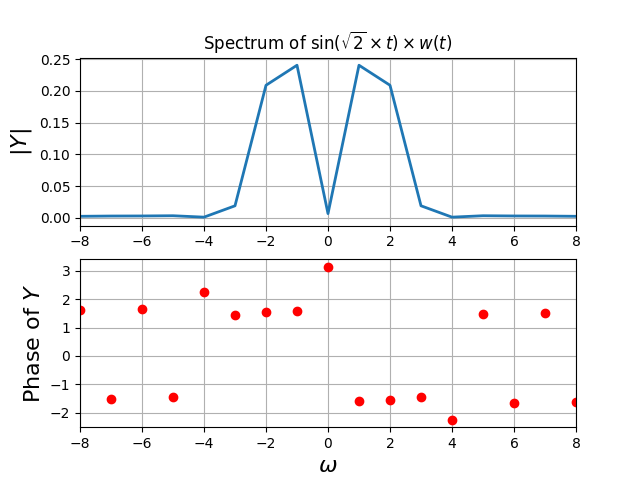
\includegraphics[scale=0.5]{Figure_6.png}
\caption{Spectrum of $sin(\sqrt{2}t)*w(t)$}
\label{fig:universe}
\end{figure}

\subsection{Spectrum of $y=\sin\left(\sqrt{2}\times t\right)\times w(t)$ with 256 samples}

The spectrum that is obtained with a time period $8\pi$ has a slightly sharper peak and is given below:
\begin{figure}[h!]
\centering
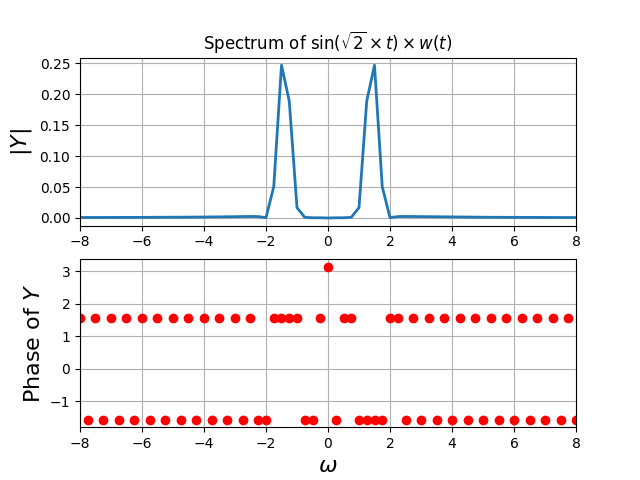
\includegraphics[scale=0.5]{Figure_7.png}
\caption{Spectrum of $sin(\sqrt{2}t)*w(t)$}
\label{fig:universe}
\end{figure}

\newpage

\section{Spectrum of $y = cos^3(w_0t)$}

\subsection{FFT without the hamming window}
\begin{figure}[h!]
\centering
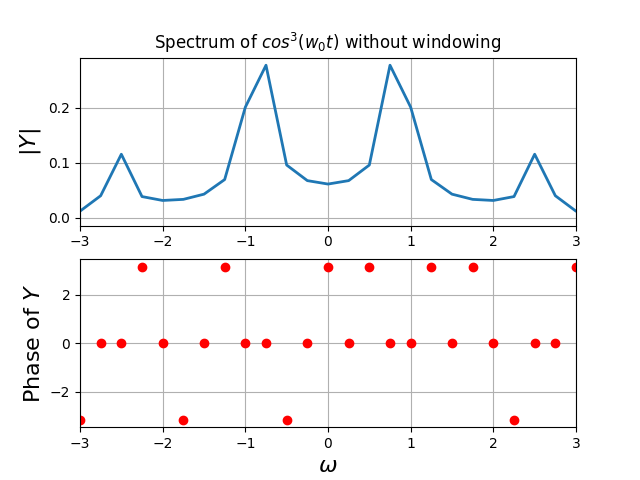
\includegraphics[scale=0.5]{Figure_8.png}
\label{fig:universe}
\end{figure}

\subsection{FFT with the hamming window}
\begin{figure}[h!]
\centering
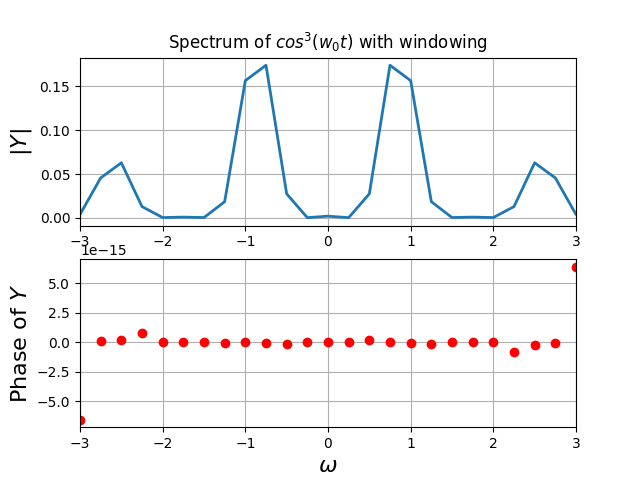
\includegraphics[scale=0.5]{Figure_9.png}
\label{fig:universe}
\end{figure}

We notice that a lot of the energy is stored in frequencies that aren't a part of the signal. After windowing, these frequencies are attenuated and hence the peaks are sharper in the windowed function. It is still not an impulse because the convolution with the Fourier transform of the windowed function smears out the peak.

\section{Spectrum of $y = cos(w_0t + \delta)$ without noise}
We need to estimate $\omega$ and $\delta$ for a signal $\cos(\omega t + \delta)$ for 128 samples between $[-\pi,\pi)$. We estimate omega using a weighted average. We have to extract the digital spectrum of the signal and find the two peaks at $\pm\omega_0$, and estimate $\omega$ and $\delta$.
\begin{figure}[h!]
\centering
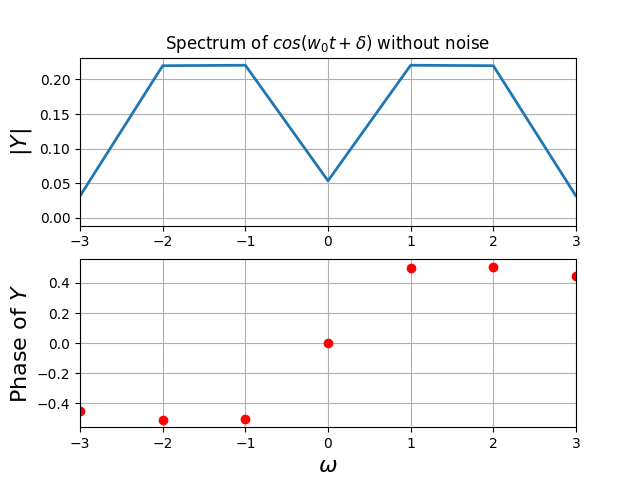
\includegraphics[scale=0.6]{Figure_10.png}
\caption{Fourier transform of $cos(1.5t+0.5)$}
\label{fig:universe}
\end{figure}

We estimate omega by performing a Mean average of $\omega$ over the magnitude of $|Y(j\omega)|$.

For delta we consider a window on each half of $\omega$ (split into positive and negative values) and extract their mean slope. The intuition behind this is that, a circular shift in the time domain of a sequence results in the linear phase of the spectra.\\\\
For true value of\\
$\omega$=1.5 and\\ 
$\delta$=0.5\\\\
Estimates for signal without noise are:\\
$\omega$: 1.5163179648582412\\
$\delta$ = 0.506776265719626

\newpage


\section{Spectrum of $y = cos(w_0t + \delta)$ with noise}
We repeat the exact same process as question 3 but with noise added to the original signal.
\begin{figure}[h!]
\centering
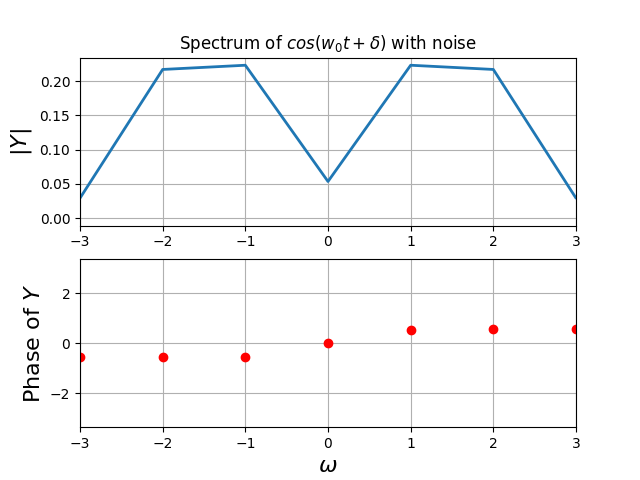
\includegraphics[scale=0.6]{Figure_11.png}
\caption{Fourier transform of noise + $cos(1.5t+0.5)$}
\label{fig:universe}
\end{figure}\\\\
For true value of\\
$\omega$=1.5 and\\ 
$\delta$=0.5\\\\
Estimates for signal with noise are:\\
$\omega$: 2.0504716417047724\\
$\delta$ = 0.5069474181511943
\newpage

\section{Chirped signal: $y = \cos\left(16\left(1.5+\frac{t}{2\pi}\right)t\right)$}
In this question we analyze a chirp signal which is an FM signal where frequency is directly proportional to time.

\subsection{FFT without Window}
\begin{figure}[h!]
\centering
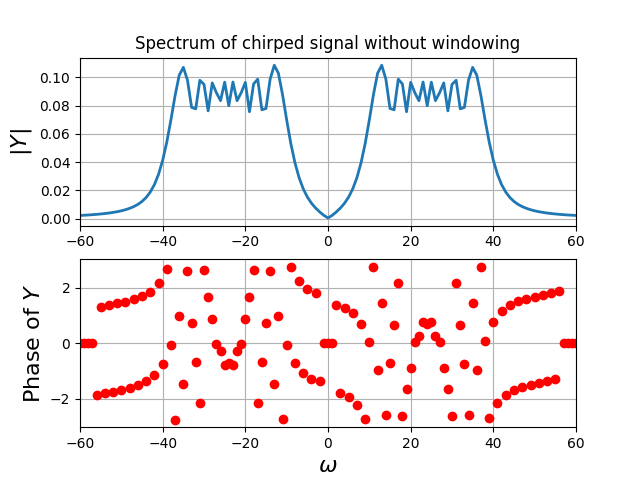
\includegraphics[scale=0.5]{Figure_12.png}
\label{fig:universe}
\end{figure}
We note that the frequency response is spread between 5-50 rad/s. A large section of this range apears due to Gibbs phenomenon. On windowing, only frequencies between 16 and 32 rad/s remain.

\subsection{FFT with Window}
\begin{figure}[h!]
\centering
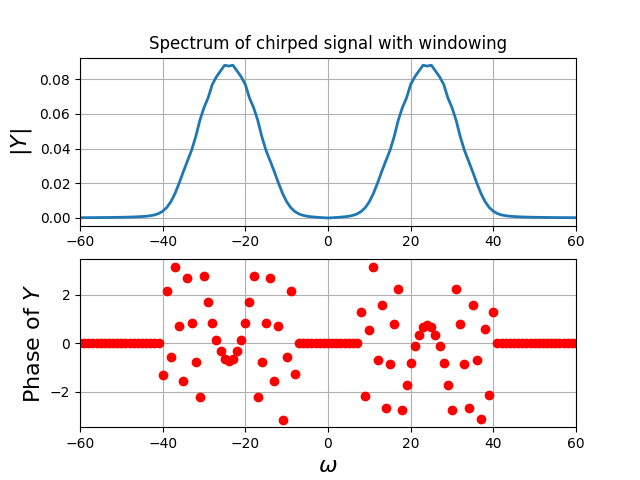
\includegraphics[scale=0.5]{Figure_13.png}
\label{fig:universe}
\end{figure}

\newpage

\section{Time-Frequency surface plot of the chirped signal: $y = \cos\left(16\left(1.5+\frac{t}{2\pi}\right)t\right)$}
For the same chirped signal, we break the 1024 vector into pieces that are 64 samples wide.
Extract the DFT of each and store as a column in a 2D array. Then plot the array as a surface plot to show how the frequency of the signal varies with time.

\begin{figure}[h!]
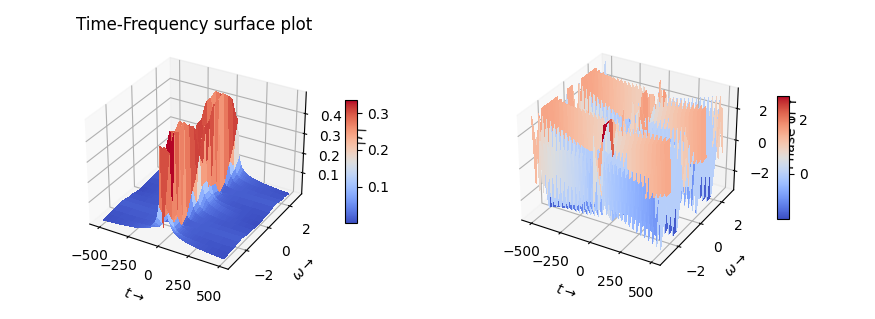
\includegraphics[scale=0.7]{Figure_14.png}
\caption{Time-Frequency surface plot}
\label{fig:universe}
\end{figure}



\section{Conclusion}
\begin{itemize}
\item In this assignment, we explore the nature of DFTs of non periodic signals,
and the use of DFT in parameter estimation.
\item These non-periodic functions have a discontinuity when periodically extended.
\item The discontinuity lead to non-harmonic components in the FFT which decay as
\(\frac{1}{\omega}\), due to Gibbs phenomenon.
\item We resolve this problem using a hamming window. It removes discontinuities by attenuating the high frequency components that cause the discontinuities. We multiply our signal with the hamming window and periodically extend it and the discontinuities nearly vanishes.
\item In the last question we analyzed a chirp signal which is an FM signal where frequency is directly proportional to time. We found that the frequency response before windowing was spread between 5-50 rad/s, but on windowing, only frequencies between 16 and 32 rad/s remain. This shows a large section of the frequency range was due to Gibbs phenomenon.


\end{itemize}



\end{document}
